%\documentclass[a4paper,11pt,fleqn,oneside, openright]{memoir} % Brug openright hvis chapters skal starte p� h�jresider; openany, oneside

%%%% PACKAGES %%%%

% �� Overs�ttelse og tegns�tning �� %
\usepackage[utf8]{inputenc}					% G�r det muligt at bruge �, � og � i sine .tex-filer
\usepackage[danish]{babel}							% Dansk sporg, f.eks. tabel, figur og kapitel
\usepackage[T1]{fontenc}								% Hj�lper med orddeling ved �, � og �. S�tter fontene til at %v�re ps-fonte, i stedet for bmp	
\usepackage{latexsym}										% LaTeX symboler
\usepackage{xcolor,ragged2e,fix-cm}			% Justering af elementer
\usepackage{pdfpages}										% G�r det muligt at inkludere pdf-dokumenter med kommandoen \includepdf[pages={x-y}]{fil.pdf}	
\pretolerance=2500 											% G�r det muligt at justre afstanden med ord (h�jt tal, mindre orddeling og mere space mellem ord)
\usepackage{ulem}                       % Gennemstregning af ord med koden \sout{}
\usepackage{fixltx2e}										% Retter forskellige bugs i LaTeX-kernen
\usepackage{gensymb}					%Tilføjer \celsius og \degree notation	
\usepackage{lineno}						%Bruges til at tilføje linjetal
																	
% �� Figurer og tabeller � floats  �� %
\usepackage{flafter}										% S�rger for at dine floats ikke optr�der i teksten f�r de er sat ind.
\usepackage{multirow}                		% Fletning af r�kker
\usepackage{hhline}                   	% Dobbelte horisontale linier
\usepackage{multicol}         	        % Fletning af kolonner
\usepackage{colortbl} 									% Mulig�re farver i tabeller
%\usepackage{float}												% G�r det muligt at placere figurer hvor du vil.   \begin{figure}[!h] % Will not be floating.
\usepackage{wrapfig}										% Inds�ttelse af figurer omsv�bt af tekst. \begin{wrapfigure}{Placering}{St�rrelse}
\usepackage{graphicx} 									% Pakke til jpeg/png billeder
\pdfoptionpdfminorversion=6							% Muligg�r inkludering af pdf dokumenter, af version 1.6 og h�jere
	
% �� Matematiske formler og maskinkode ��
\usepackage{amsmath,amssymb,stmaryrd} 	% Bedre matematik og ekstra fonte
\usepackage{textcomp}                 	% Adgang til tekstsymboler
\usepackage{mathtools}									% Udvidelse af amsmath-pakken. 
\usepackage{eso-pic}										% Tilf�j billedekommandoer p� hver side
\usepackage{lipsum}											% Dummy text \lipsum[..]
\usepackage{rsphrase}										% Kemi-pakke til RS-s�tninger
\usepackage[version=3]{mhchem} 					% Kemi-pakke til lettere notation af formler

% �� Referencer, bibtex og url'er �� %
\usepackage{url}												% Til at s�tte urler op med. Virker sammen med hyperref
\usepackage[danish]{varioref}						% Giver flere bedre mulighed for at lave krydshenvisninger
\usepackage{natbib}											% Litteraturliste med forfatter-�r og nummerede referencer
\usepackage{xr}													% Referencer til eksternt dokument med \externaldocument{<NAVN>}

% �� Floats �� %
%\let\newfloat\relax 										% Memoir har allerede defineret denne, men det g�r float pakken ogs�
%\usepackage{float}

\usepackage[footnote,draft,danish,silent,nomargin]{fixme}		% Inds�t rettelser og lignende med \fixme{...} Med final i stedet for draft, udl�ses en error 																															for hver fixme, der ikke er slettet, n�r rapporten bygges.

%%%% CUSTOM SETTINGS %%%%

% �� Marginer �� %
\setlrmarginsandblock{3.5cm}{2.5cm}{*}	% \setlrmarginsandblock{Indbinding}{Kant}{Ratio}
\setulmarginsandblock{2.5cm}{3.0cm}{*}	% \setulmarginsandblock{Top}{Bund}{Ratio}
\checkandfixthelayout 									% Laver forskellige beregninger og s�tter de almindelige l�ngder op til brug ikke memoir pakker

%	�� Afsnitsformatering �� %
\setlength{\parindent}{0mm}           	% St�rrelse af indryk
\setlength{\parskip}{4mm}          			% Afstand mellem afsnit ved brug af double Enter
\linespread{1,1}												% Linie afstand

% �� Litteraturlisten �� %
\bibpunct[,]{[}{]}{;}{a}{,}{,} 					% Definerer de 6 parametre ved Harvard henvisning (bl.a. parantestype og seperatortegn)
%\bibliographystyle{bibtex/harvard}			% Udseende af litteraturlisten. Ligner dk-apali - mvh Klein

% �� Indholdsfortegnelse �� %
\setsecnumdepth{subsection}		 					% Dybden af nummerede overkrifter (part/chapter/section/subsection)
\maxsecnumdepth{subsection}							% �ndring af dokumentklassens gr�nse for nummereringsdybde
\settocdepth{section} 								% Dybden af indholdsfortegnelsen

% �� Visuelle referencer �� %
\usepackage[colorlinks=true]{hyperref}			 	% Giver mulighed for at ens referencer bliver til klikbare hyperlinks. .. [colorlinks]{..}
\hypersetup{pdfborder = 0}							% Fjerner ramme omkring links i fx indholsfotegnelsen og ved kildehenvisninger ��
\hypersetup{														%	Ops�tning af farvede hyperlinks
    colorlinks = true,
    linkcolor = black,
    anchorcolor = black,
    citecolor = black,
    urlcolor = black
}

\definecolor{gray}{gray}{0.80}					% Definerer farven gr�

% �� Ops�tning af figur- og tabeltekst �� %
 	\captionnamefont{
 		\small\bfseries\itshape}						% Ops�tning af tekstdelen ("Figur" eller "Tabel")
  \captiontitlefont{\small}							% Ops�tning af nummerering
  \captiondelim{. }											% Seperator mellem nummerering og figurtekst
  \hangcaption													%	Venstrejusterer flere-liniers figurtekst under hinanden
  \captionwidth{\linewidth}							% Bredden af figurteksten
	\setlength{\belowcaptionskip}{10pt}		% Afstand under figurteksten
		
% �� Navngivning �� %
\addto\captionsdanish{
	\renewcommand\appendixname{Appendiks}
	\renewcommand\contentsname{Indholdsfortegnelse}	
	\renewcommand\appendixpagename{Appendiks}
%	\renewcommand\cftchaptername{\chaptername~}				% Skriver "Kapitel" foran kapitlerne i indholdsfortegnelsen
	\renewcommand\cftappendixname{\appendixname~}			% Skriver "Appendiks" foran bilagene i indholdsfortegnelsen
	\renewcommand\appendixtocname{Appendiks}
}

% �� Kapiteludssende �� %
\definecolor{numbercolor}{gray}{0.7}			% Definerer en farve til brug til kapiteludseende
\newif\ifchapternonum

\makechapterstyle{jenor}{									% Definerer kapiteludseende -->
  \renewcommand\printchaptername{}
  \renewcommand\printchapternum{}
  \renewcommand\printchapternonum{\chapternonumtrue}
  \renewcommand\chaptitlefont{\fontfamily{pbk}\fontseries{db}\fontshape{n}\fontsize{25}{35}\selectfont\raggedleft}
  \renewcommand\chapnumfont{\fontfamily{pbk}\fontseries{m}\fontshape{n}\fontsize{1in}{0in}\selectfont\color{numbercolor}}
  \renewcommand\printchaptertitle[1]{%
    \noindent
    \ifchapternonum
    \begin{tabularx}{\textwidth}{X}
    {\let\\\newline\chaptitlefont ##1\par} 
    \end{tabularx}
    \par\vskip-2.5mm\hrule
    \else
    \begin{tabularx}{\textwidth}{Xl}
    {\parbox[b]{\linewidth}{\chaptitlefont ##1}} & \raisebox{-15pt}{\chapnumfont \thechapter}
    \end{tabularx}
    \par\vskip2mm\hrule
    \fi
  }
}																						% <--

\chapterstyle{jenor}												% Valg af kapiteludseende - dette kan udskiftes efter �nske

% �� Sidehoved �� %

%\makepagestyle{custom}																				% Definerer sidehoved og sidefod - kan modificeres efter �nske -->
%\makepsmarks{custom}{																						
%\def\chaptermark##1{\markboth{\itshape\thechapter. ##1}{}}		% Henter kapitlet den p�g�ldende side h�rer under med kommandoen \leftmark. \itshape g�r teksten kursiv
%\def\sectionmark##1{\markright{\thesection. ##1}{}}					% Henter afsnittet den p�g�ldende side h�rer under med kommandoen \rightmark
%}																														% Sidetallet skrives med kommandoen \thepage	
%\makeevenhead{custom}{Gruppe B130}{}{\leftmark}							% Definerer lige siders sidehoved efter modellen \makeevenhead{Navn}{Venstre}{Center}{H�jre}
%\makeoddhead{custom}{\rightmark}{}{Aalborg Universitet}			% Definerer ulige siders sidehoved efter modellen \makeoddhead{Navn}{Venstre}{Center}{H�jre}
%\makeevenfoot{custom}{\thepage}{}{}													% Definerer lige siders sidefod efter modellen \makeevenfoot{Navn}{Venstre}{Center}{H�jre}
%\makeoddfoot{custom}{}{}{\thepage}														% Definerer ulige siders sidefod efter modellen \makeoddfoot{Navn}{Venstre}{Center}{H�jre}		
%\makeheadrule{custom}{\textwidth}{0.5pt}											% Tilf�jer en streg under sidehovedets indhold
%\makefootrule{custom}{\textwidth}{0.5pt}{1mm}								% Tilf�jer en streg under sidefodens indhold

%\copypagestyle{nychapter}{custom}														% F�lgende linier s�rger for, at sidefoden bibeholdes p� kapitlets f�rste side
%\makeoddhead{nychapter}{}{}{}
%\makeevenhead{nychapter}{}{}{}
%\makeheadrule{nychapter}{\textwidth}{0pt}
%\aliaspagestyle{chapter}{nychapter}													% <--

\pagestyle{plain}																							% Valg af sidehoved og sidefod

% �� Fjerner den vertikale afstand mellem listeopstillinger og punktopstillinger �� %
\let\olditemize=\itemize							
\def\itemize{\olditemize\setlength{\itemsep}{-1ex}}
\let\oldenumerate=\enumerate						
\def\enumerate{\oldenumerate\setlength{\itemsep}{-1ex}}

%%%% CUSTOM COMMANDS %%%%

% �� Billede hack �� %
\newcommand{\figur}[4]{
		\begin{figure}[H] \centering
			\includegraphics[width=#1\textwidth]{billeder/#2}
			\caption{#3}\label{#4}
		\end{figure} 
}

% �� Specielle tegn �� %
\newcommand{\grader}{^{\circ}C}
\newcommand{\gr}{^{\circ}}
\newcommand{\g}{\cdot}

% �� Promille-hack (\promille) �� %
\newcommand{\promille}{%
  \relax\ifmmode\promillezeichen
        \else\leavevmode\(\mathsurround=0pt\promillezeichen\)\fi}
\newcommand{\promillezeichen}{%
  \kern-.05em%
  \raise.5ex\hbox{\the\scriptfont0 0}%
  \kern-.15em/\kern-.15em
  \lower.25ex\hbox{\the\scriptfont0 00}}

%%%% ORDDELING %%%%

\hyphenation{hvad hvem hvor}

%%%% Tabeler %%%%
\usepackage{threeparttable}
\usepackage[tableposition=top]{caption}

%%%% listings %%%%
\usepackage{listings}
\lstset{language=C}
\lstset{backgroundcolor=,rulecolor=}
\lstset{commentstyle=\textit}
\usepackage{lastpage}

\usepackage{marvosym}

%%%% top/tail %%%%

%\newcommand{\toptail}[1]{\fboxsep2mm\fbox{\begin{minipage}{145.3mm}#1\end{minipage}}}

\newcommand{\Ohm}{\ohm}
\newcommand{\my}{\mu}
\newcommand{\kilde}[1]{\fixme{Kilde: #1}}

 \usepackage[electronic]{ifsym}
%\begin{document}
\chapter{Appendiks E}
\label{maalejournal_indgangsvaelger}
\section*{Måling på indgangsvælger}
Denne målerapport dokumenterer målinger foretaget på projektets indgangsvaelger, opbygget som beskrevet i kapitel \ref{forforstaerker}. Målingen er foretaget på Fredrik Bajers Vej 7 i lokale B1-104 på Aalborg Universitet den 14. december 2010 af gruppe 311.

\subsection*{Formål}
\label{maalejournal_formaal}
Målingens formål er at:
\begin{itemize}
\item Kontrollere funktionen af indgangsvælgeren og finde evt. fejl
\item Måle dæmpningen for en tændt samt en slukket indgang i indgangsvælgeren.
\item Måle outputtet i forhold til hvor mange indgange der er valgt .
\item Måle indgangsimpedansen for indgangene, tændt og slukket.
\item Måle at frekvensgangen ved 20 Hz - 20 kHz 
\end{itemize}

\subsection*{Testobjekt}
\label{maalejournal_testobjekt}
Der vil i denne målerapport blive udført tests af indgangsvælgeren. Indgangsimpedansen måles for alle indgangene: De to stereo indgange og mikrofon indgangen. Alle indgangsimpedanserne måles for både en tændt og en slukket indgang.
Til frekvensmåling 
\begin{figure}[h]
\centering
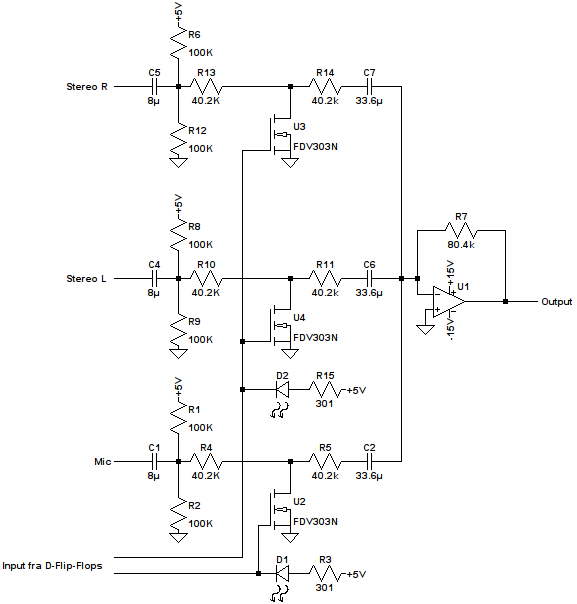
\includegraphics[scale=0.8]{maalerapporter/indgangsvaelger/indgangvaelger_ltspice_diagram.png}
\caption{Diagram over kredsløbet der testes.}
\label{maalerap-diagram_simulering}
\end{figure}

\subsection*{Teori}
\label{maalejournal_teori}
Teorien bag en impedansmåling, er at der skabes en spændingsdeling mellem en kendt reference modstand og indgangsmodstanden i det testede. Forholdet af spændingerne som ligger over modstandene svarer til forholdet mellem modstandene.

\subsection*{Måleopstilling}
\label{maalejournal_maaleopstilling}
Måleopstillingerne er vist på figur \ref{fig:indgang:maaleop-thd} .

\begin{figure}[h]
\centering
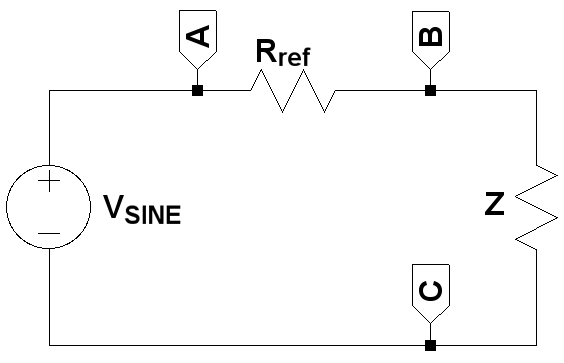
\includegraphics[scale=0.4]{maalerapporter/indgangsvaelger/impedansopstilling-forforstaerker.png}
\caption{Måleopstilling for impedansmåling}
\label{fig:indgang:maaleop-imp}
\end{figure}

\begin{figure}[h]
\centering
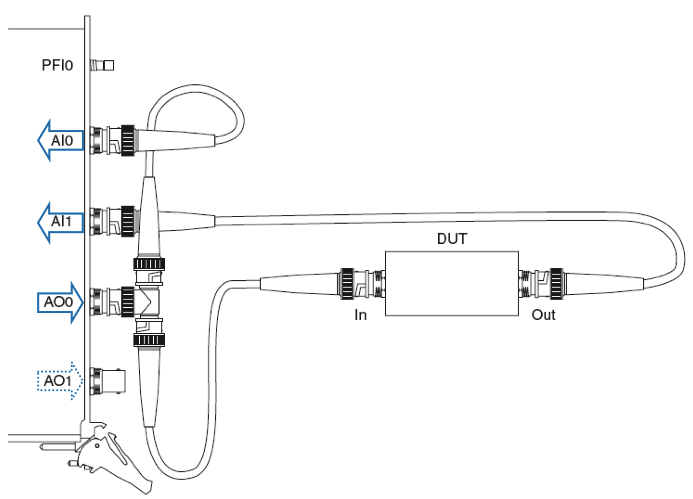
\includegraphics[scale=0.4]{maalerapporter/indgangsvaelger/maaleopstilling-thd-forforstaerker.png}
\caption{Måleopstilling for forstærkning-, frekvensgang- og forvrængningsmåling}
\label{fig:indgang:maaleop-thd}
\end{figure}

\subsection*{Anvendt udstyr}
\label{indgang:maalejournal_anvendtudstyr}

\begin{table}[h]
\centering
\begin{tabular}{l|c|l}
\hline\hline
Instrument & AAU-nr. & Fabrikant, type m.v. \\
\hline\hline
Oscilloskop & 33866 & Agilent 54621A \\[4pt]
Oscillator & 07995 & B\&O RC-oscillator TG7 \\[4pt]
Spændingsforsyning & 39897 & HAMEG HM7042 \\[4pt]
Spændingsforsyning & 33901 & HAMEG HM7042 \\[4pt]
Multimeter & 33048 & Fluke and Philips FLUKE 37 \\[4pt]
Multimeter & 08518 & Fluke and Philips FLUKE 37 \\[4pt]
Audioanalysator & 76986 & National Instruments NI-PCI-4461 \\
\hline\hline
\end{tabular}
\label{tab:indgang:maaleudstyr_forforstaerker}
\end{table}

\subsection*{Måleprocedure}
\label{indgang:maalejournal_maaleprocedure}
Proceduren for impedansmålingen er:

\begin{enumerate}
\item Generatoren, kaldet $V_\mathrm{SINE}$ på figur \ref{fig:indgang:maaleop-imp}, indstilles til en effektivspænding på 21,1 mV (indstilles med oscilloskop) ved 1 kHz og tilsluttes
\item Reference modstanden, kaldet $R_\mathrm{ref}$ på figur \ref{fig:indgang:maaleop-imp}, vælges til 10 k\ohm~ og tilsluttes
\item Spændingsfaldet fra terminal A til terminal B, som på figur \ref{fig:fig:indgang:maaleop-imp}, måles
\item Spændingsfaldet fra terminal B til terminal C, som på figur \ref{fig:fig:indgang:maaleop-imp}, måles
\end{enumerate}
Herefter slukkes for indgang, og målingen foretages igen. Dette gentages for hver indgang.

Proceduren for forstærkning-, frekvensgang- og forvrængningsmålingen er:

\begin{enumerate}
\item En spændingsforsyning indstilles til $\pm15~V$ (indstilles med multimeteret) og tilsluttes.
\item En spændingsforsyning indstilles til 5 V (indstilles med multimeteret) og tilsluttes.
\item Testobjektet tilsluttes som på figur \ref{fig:indgang:maaleop-thd}
\item Kanalen der måles på, indstilles ved hjælp af trykknappen.
\item Programmet $"$Swept Sine - Linear Response and Harmonic Distortion (DAQmx)$"$ startes
\item $"$Start frequency$"$ under Source settings sættes til 20 Hz
\item $"$Stop frequency$"$ under Source settings sættes til 20 kHz
\item $"$Amplitude$"$ under Source settings sættes til 2 V
\item $"$THD units$"$ sættes til \%
\item $"$AI Range$"$ for Stimulus channel sættes til $\pm$ 0,316 V\fixme{Check}
\item $"$AI Range$"$ for Respons channel sættes til $\pm$ 3,16 V\fixme{dem her}
\item $"$Sampling frequency$"$ sættes til 204,8 kHz
\end{enumerate}

Samme procedure gennemføres, hvor amplituden i punkt 7 i stedet sættes til 200 mV. Dermed opnåes resultater for både maksimums- og minimumsinput. 

\subsection*{Resultater}
\label{maalejournal_resultater}


Impedansmålingen gav effektivspændingerne vist i tabel \ref{tab:resultatimpedans_indgang}. Disse spændinger bruges til at regne testobjektets indgangsimpedans, med formel (\ref{equ:zresultat-indgang})\fixme{kilde: Ole Kiel Jensen, mm4 Maaleteknik}.

\begin{equation}
\label{equ:zresultat-indgang}
\vert Z \vert = \frac{\vert V_Z \vert}{\vert V_{R_\mathrm{ref}} \vert} \cdot R_\mathrm{ref}
\end{equation} 

\begin{table}[h]
\centering
\begin{tabular}{l|c|c|l}

\hline\hline
\multicolumn{4}{c}{\textbf{Mikrofon Indgang}} \\
\hline\hline
& Målt værdi & Beregnet værdi & Enhed \\
\hline\hline
Tændt: $V_{R_\mathrm{ref}}$ & 5,1& & mV effektiv\\[4pt]
Tændt: $V_Z$ & 16,1 & & mV effektiv\\[4pt]
Tændt: $R_\mathrm{i,forforstaerker}$ & & 31,56 & k\ohm \\
Slukket: $V_{R_\mathrm{ref}}$ & 6,5& & mV effektiv\\[4pt]
Slukket: $V_Z$ & 14,7 & & mV effektiv\\[4pt]
Slukket: $R_\mathrm{i,forforstaerker}$ & & 22,62 & k\ohm \\
\hline\hline
\multicolumn{4}{c}{} \\
\hline\hline
\multicolumn{4}{c}{\textbf{Stereo L}} \\
\hline\hline
& Målt værdi & Beregnet værdi & Enhed \\
\hline\hline
Tændt: $V_{R_\mathrm{ref}}$ & 5,1& & mV effektiv\\[4pt]
Tændt: $V_Z$ & 16,1 & & mV effektiv\\[4pt]
Tændt: $R_\mathrm{i,forforstaerker}$ & & 31,56 & k\ohm \\
Slukket: $V_{R_\mathrm{ref}}$ & 6,5& & mV effektiv\\[4pt]
Slukket: $V_Z$ & 14,7 & & mV effektiv\\[4pt]
Slukket: $R_\mathrm{i,forforstaerker}$ & & 22,62 & k\ohm \\
\hline\hline
\multicolumn{4}{c}{} \\
\hline\hline
\multicolumn{4}{c}{\textbf{Stereo R}} \\
\hline\hline
& Målt værdi & Beregnet værdi & Enhed \\
\hline\hline
Tændt: $V_{R_\mathrm{ref}}$ & 5,1& & mV effektiv\\[4pt]
Tændt: $V_Z$ & 16,1 & & mV effektiv\\[4pt]
Tændt: $R_\mathrm{i,forforstaerker}$ & & 31,56 & k\ohm \\
Slukket: $V_{R_\mathrm{ref}}$ & 6,5& & mV effektiv\\[4pt]
Slukket: $V_Z$ & 14,7 & & mV effektiv\\[4pt]
Slukket: $R_\mathrm{i,forforstaerker}$ & & 22,62 & k\ohm \\
\hline\hline
\end{tabular}
\caption{Resultater af impedansmåling}
\label{tab:resultatimpedans_indgang}
\end{table}

Frekvensgangen og THD blev målt for de forskellige indgange. Resultaterne er vist i figur \ref{fig:apind:frek200mv} til figur \ref{fig:apind:thd2vslukket}. Resten af resultaterne kan findes på CD'en\fixme{henvisning}. Spændingsniveauer angivet i V og mV er amplitude værdier. 


\begin{figure}[h]
\centering
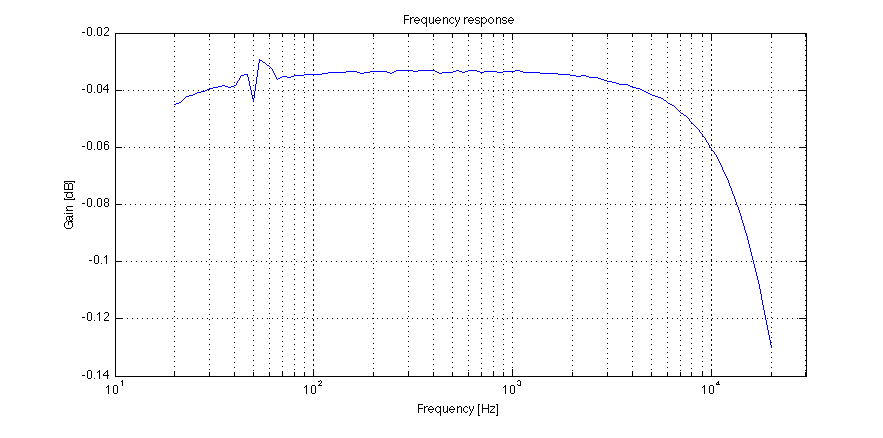
\includegraphics[width=\textwidth]{maalerapporter/indgangsvaelger/Indgangsvlger mic 200mv frek.png}
\caption{Frekvensgangen for mikrofonindgangen på indgangsvælgeren ved 200 mV.}
\label{fig:apind:frek200mv}
\end{figure}


\begin{figure}[h]
\centering
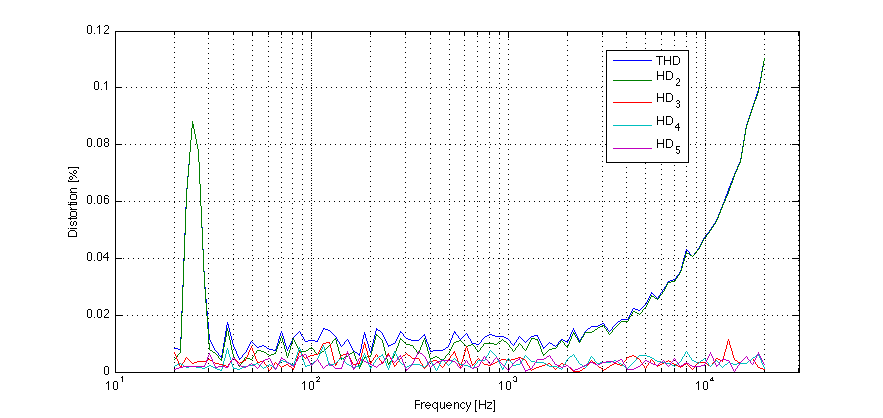
\includegraphics[width=\textwidth]{maalerapporter/indgangsvaelger/Indgangsvlger mic 200mv thd.png}
\caption{THD for mikrofonindgangen på indgangsvælgeren ved 200 mV.}
\label{fig:apind:thd200mv}
\end{figure}


\begin{figure}[h]
\centering
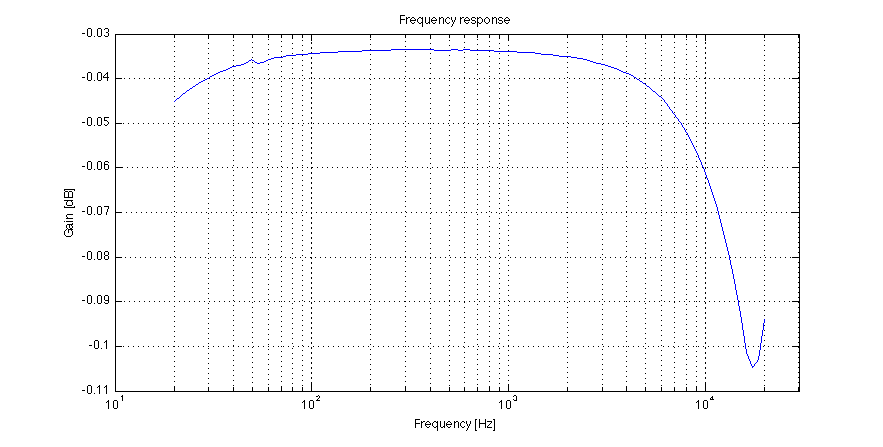
\includegraphics[width=\textwidth]{maalerapporter/indgangsvaelger/Indgangsvlger mic 2v frek.png}
\caption{Frekvensgangen for mikrofonindgangen på indgangsvælgeren ved 2V.}
\label{fig:apind:frek2v}
\end{figure}


\begin{figure}[h]
\centering
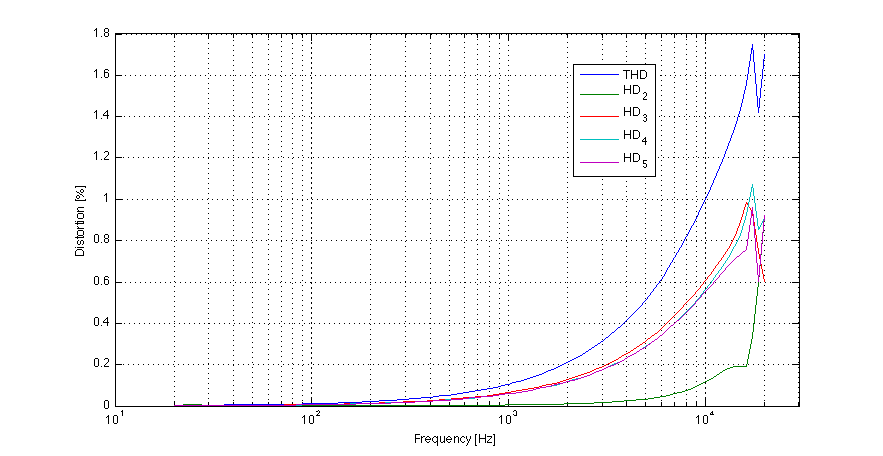
\includegraphics[width=\textwidth]{maalerapporter/indgangsvaelger/Indgangsvlger mic 2v thd.png}
\caption{THD for mikrofonindgangen på indgangsvælgeren ved 2 V.}
\label{fig:apind:thd2v}
\end{figure}


\begin{figure}[h]
\centering
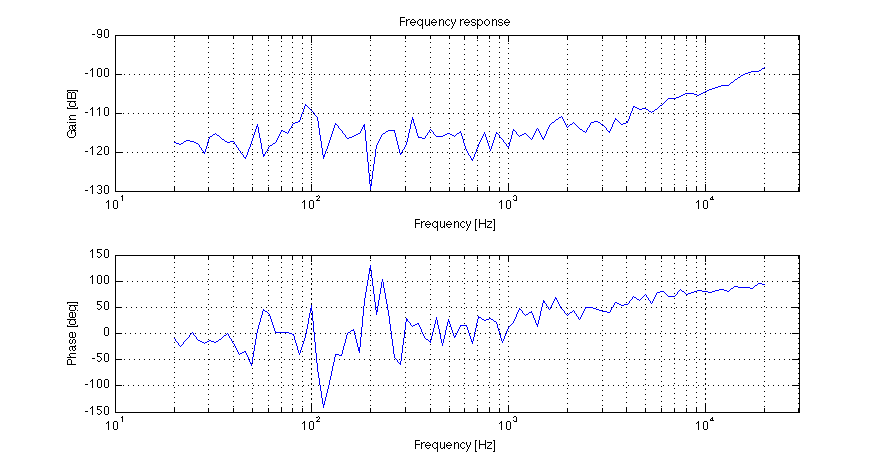
\includegraphics[width=\textwidth]{maalerapporter/indgangsvaelger/Indgangsvlger mic 2v slukket frek.png}
\caption{Frekvensgangen og fasedrejet for mikrofonindgangen for et slukket signal, på indgangsvælgeren ved 2V.}
\label{fig:apind:frek2vslukket}
\end{figure}


\begin{figure}[h]
\centering
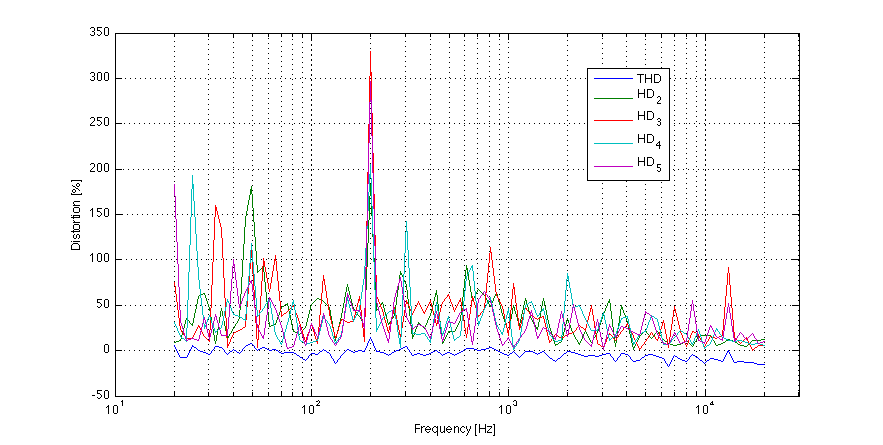
\includegraphics[width=\textwidth]{maalerapporter/indgangsvaelger/Indgangsvlger mic 2v slukket thd.png}
\caption{THD for mikrofonindgangen for et slukket signal, på indgangsvælgeren ved 2 V.}
\label{fig:apind:thd2vslukket}
\end{figure}

\subsection*{Måleusikkerheder}
\label{maalejournal_maaleusikkerheder}
De væsentligste usikkerheder er:
\begin{itemize}
\item Komponent tolerancer
\item Påvirkning fra måleinstrument
\item Måleinstrument unøjagtighed
\item Støj, 50 Hz brum
\item Anden indstråling
\end{itemize}

%\end{document}